\documentclass[ ../main.tex]{subfiles}
\providecommand{\mainx}{..}
\begin{document}
\section{Random approximate set model}
\label{sec:asets}
% NOTE: there is another random Boolean algebra model where
% the universe is an approximate set of U. 
The concept of a random approximate set depends upon the concept of an \emph{approximate set}.

Given an objective set $\Set{S}$, any element that is a member of $\Set{S}$ is denoted a \emph{positive} of $\Set{S}$ and any element that is \emph{not} a member of $\Set{S}$ is denoted a \emph{negative} of $\Set{S}$.

A set that is used as an \emph{approximation} of $\Set{S}$ may be denoted by $\ASet{S}$.
If the \emph{only} information we have about $\Set{S}$ is given by $\ASet{S}$, then we may perform membership tests on $\ASet{S}$ to \emph{predict} the members (or non-members) of $\Set{S}$.

There are two ways a binary prediction can be false.
\begin{enumerate}
    \item A \emph{false positive} occurs if a negative of the objective set is predicted to be a positive. False positives are also known as \emph{type I errors}.
    The complement of false positives are \emph{true negatives}.
    \item A \emph{false negative} occurs if a positive of the objective set is predicted to be a negative. False negatives are also known as \emph{type II errors}.
    The complement of false negatives are \emph{true positives}.
\end{enumerate} 

Suppose we have an objective set $\Set{S}$ and an approximation $\ASet{S}$.
If we denote the set of false positives by $\Set{F}[p]$, true positives by $\Set{T}[p]$, false negatives by $\Set{F}[n]$, and true negatives by $\Set{T}[n]$, then the objective set $\Set{S}$ is equal to $\SetUnion[\Set{F}[n]][\Set{T}[p]]$ and the approximate set $\ASet{S}$ is equal to $\SetUnion[\Set{T}[p]][\Set{F}[p]]$.
See \cref{fig:ex_approx_set} for an illustration.
\begin{figure}[ht]
\caption{An approximate set $\ASet{S}$ of an objective set $\Set{S}$}
\label{fig:ex_approx_set}
\centering
\def\svgwidth{\columnwidth/2}
%% Creator: Inkscape inkscape 0.92.1, www.inkscape.org
%% PDF/EPS/PS + LaTeX output extension by Johan Engelen, 2010
%% Accompanies image file 'aset_fp_fn.pdf' (pdf, eps, ps)
%%
%% To include the image in your LaTeX document, write
%%   \input{<filename>.pdf_tex}
%%  instead of
%%   \includegraphics{<filename>.pdf}
%% To scale the image, write
%%   \def\svgwidth{<desired width>}
%%   \input{<filename>.pdf_tex}
%%  instead of
%%   \includegraphics[width=<desired width>]{<filename>.pdf}
%%
%% Images with a different path to the parent latex file can
%% be accessed with the `import' package (which may need to be
%% installed) using
%%   \usepackage{import}
%% in the preamble, and then including the image with
%%   \import{<path to file>}{<filename>.pdf_tex}
%% Alternatively, one can specify
%%   \graphicspath{{<path to file>/}}
%% 
%% For more information, please see info/svg-inkscape on CTAN:
%%   http://tug.ctan.org/tex-archive/info/svg-inkscape
%%
\begingroup%
  \makeatletter%
  \providecommand\color[2][]{%
    \errmessage{(Inkscape) Color is used for the text in Inkscape, but the package 'color.sty' is not loaded}%
    \renewcommand\color[2][]{}%
  }%
  \providecommand\transparent[1]{%
    \errmessage{(Inkscape) Transparency is used (non-zero) for the text in Inkscape, but the package 'transparent.sty' is not loaded}%
    \renewcommand\transparent[1]{}%
  }%
  \providecommand\rotatebox[2]{#2}%
  \ifx\svgwidth\undefined%
    \setlength{\unitlength}{437.78998862bp}%
    \ifx\svgscale\undefined%
      \relax%
    \else%
      \setlength{\unitlength}{\unitlength * \real{\svgscale}}%
    \fi%
  \else%
    \setlength{\unitlength}{\svgwidth}%
  \fi%
  \global\let\svgwidth\undefined%
  \global\let\svgscale\undefined%
  \makeatother%
  \begin{picture}(1,1.05361373)%
    \put(-0.00881474,0.603155){\color[rgb]{0,0,0}\makebox(0,0)[lb]{\smash{}}}%
    \put(-0.01615682,0.61783922){\color[rgb]{0,0,0}\makebox(0,0)[lb]{\smash{}}}%
    \put(0,0){\includegraphics[width=\unitlength,page=1]{aset_fp_fn.pdf}}%
    \put(0.78,0.06){\color[rgb]{0,0,0}\makebox(0,0)[lb]{\smash{$\Set{S} = \SetUnion[\Set{T}[p]][\Set{F}[n]]$}}}%
    \put(0.01737703,1.02584642){\color[rgb]{0,0,0}\makebox(0,0)[lb]{\smash{$\ASet{S} = \SetUnion[\Set{T}[p]][\Set{F}[p]]$}}}%
    \put(0.67844448,0.84067833){\color[rgb]{0,0,0}\makebox(0,0)[lb]{\smash{$\Set{F}[p]$}}}%
    \put(0.84976816,0.43053962){\color[rgb]{0,0,0}\makebox(0,0)[lb]{\smash{$\Set{F}[n]$}}}%
    \put(0.50885122,0.45649776){\color[rgb]{0,0,0}\makebox(0,0)[lb]{\smash{$\Set{T}[p]$}}}%
    \put(0.03987408,0.45476734){\color[rgb]{0,0,0}\makebox(0,0)[lb]{\smash{$\Set{T}[n]$}}}%
    \put(0,0){\includegraphics[width=\unitlength,page=2]{aset_fp_fn.pdf}}%
  \end{picture}%
\endgroup%

\end{figure}

If we only have access to the approximation $\ASet{S}$, we cannot partition the universe into the sets $\Set{F}[p]$, $\Set{T}[p]$, $\Set{F}[n]$, and $\Set{T}[n]$ as demonstrated in \cref{fig:ex_approx_set}.
However, we can quantify the degree of \emph{uncertainty} about the elements that are predicted to be positive or negative.

The false positive and true negative \emph{rates} are given by the following.
\begin{definition}
\label{def:fprate}
The \emph{false positive rate} is the proportion of predictions that are \emph{false positives} as given by
\begin{equation}
     \fprateob = \frac{f_p}{f_p + t_n}\,,
\end{equation}
where $f_p$ is the number of \emph{false positives} and $t_n$ is the number of  \emph{true negatives}.
In a complementary manner, the \emph{true negative rate} is $\tnrateob = 1 - \fprateob$.
\end{definition}

The true positive and false negative \emph{rates} are given by the following.
\begin{definition}
The \emph{true positive rate} is the proportion of predictions that are \emph{true positives} as given by
\begin{equation}
\tprateob = \frac{t_p}{t_p + f_n}\,,
\end{equation}
where $f_n$ is the number of \emph{false negatives} and $t_p$ is the number of \emph{true positives}.
In a complementary manner, the \emph{false negative rate} is $\fnrateob = 1 - \tprateob$.
\end{definition}

The \emph{probabilities} of the four possible predictive outcomes are given by 
\cref{tbl:contingency_table}.
\begin{table}[ht]
\centering
\begin{tabular}{@{} l l l @{}}
    \toprule
    & \textbf{positive} & \textbf{negative}\\
    \midrule
    \textbf{predict positive} & $\tprateob=1-\fnrateob$ & 
    $\fprateob=1-\tnrateob$\\
    \textbf{predict negative} & $\fnrateob=1-\tprateob$ & 
    $\tnrateob=1-\fprateob$\\
    \bottomrule
\end{tabular}
\caption{The $2 \times 2$ contingency table of outcomes for approximate sets.}
\label{tbl:contingency_table}        
\end{table}

In the \emph{random} approximate set model, we do not describe any particular approximation, but rather we describe the statistical properties of 
processes that \emph{generate} approximations.

The random false positive rate $\FPR$ and false negative rate $\FNR$ have supports in the Borel set of $[0,1]$.

The \emph{zero-th order} generative model for sets is not generally known, but we denote the zero-th order model by $\RV{R}$.
We denote the \emph{first-order} random approximate set generative model by $\AT{\RV{R}}$.
The joint distribution of $\AT{\RV{R}}$, $\FPR$, $\FNR$, and $\RV{R}$ given a unviersal set $\Set{U}$ has a probability density
\begin{equation}
\PDF{\Set{Y}, \fprate, \fnrate, \Set{X} \Given \Set{U}}[\AT{\RV{R}}, \FPR, \FNR, \RV{R}]\,.
\end{equation}
By the axioms of probability theory, this may be decomposed into
\begin{equation}
\PDF{\Set{Y},\fprate, \fnrate, \Set{X} \Given \Set{U}}[\AT{\RV{R}}, \FPR, \FNR, \RV{R}] =
\PDF{\Set{Y} \Given \fprate, \fnrate, \Set{X} \Given \Set{U}}[\AT{\RV{R}} \Given \FPR, \FNR, \RV{R}]
\PDF{\fprate, \fnrate \Given \Set{X}}[\FPR, \FNR \Given \RV{R}]
\PDF{\Set{X} \Given \Set{U}}[\RV{R}]\,.
\end{equation}
We typically omit the explicit reference to $\Set{U}$, since it may usually be understood as implicit to the model.

The object of central interest is the distribution of $\AT{\RV{R}}$ given $\RV{R}$.
The conditional distribution of $\AT{\RV{R}}$ given $\RV{R} = \Set{X}$ is denote by $\ASet{X}$.
By the axioms of probability,
\begin{equation}
\PDF{\Set{Y},\fprate, \fnrate}[\ASet{X}, \FPR, \FNR] =
\PDF{\Set{Y} \Given \fprate, \fnrate}[\ASet{X} \Given \FPR, \FNR]
\PDF{\fprate, \fnrate \Given \Set{X}}[\FPR, \FNR \Given \RV{R}]\,.
\end{equation}


The random false positive and false negative rates conditioned on $\RV{R} = \Set{X}$ are respectively given by
\begin{equation}
\FPR = \frac{1}{\Card{\Set{X}}} \sum_{x \in \SetComplement[\Set{X}]} \SetIndicator{\ASet{X}}(x)
\end{equation}
and
\begin{equation}
\FNR = \frac{1}{\Card{\SetComplement[\Set{X}]}} \sum_{x \in \Set{X}} \SetIndicator{\ASet{X}}(x)\,.
\end{equation}

$\ASet{A}$ conditioned on $\FPR = a$ and $\FNR = b$ is a random approximate set with the indicated false positive and false negative rates.
If the rates happen to pick out a specific set in the support, then the result is a degenerate distribution, e.g., $\ASet{A}$ given $\FPR = 0$ and $\FNR = 0$ is degenerate where all probability mass is assigned to $\Set{A}$.

We denote the distributions of $\ASet{X}$ given $\Expect{\FPR} = \fprate$ and $\ASet{X}$ given $\Expect{\FNR} = \fnrate$ respectively by $\ASet{X}[\fprate][-]$ and $\ASet{X}[+][\fnrate]$.
An object of central interest is the distribution of $\ASet{X}$ given $\Expect{\FPR} = \fprate$ and $\Expect{\FNR} = \fnrate$, denoted by
\begin{equation}
\ASet{X}[\fprate][\fnrate]\,.
\end{equation}

If we \emph{sample} from $\ASet{A}[\fprate][\fnrate]$, some set $\Set{Y} \in \PS{\Set{U}}$ with false positive rate $a$ and false negative rate $b$ will be realized with probability $\PDF{\Set{Y} \Given a, b}[\ASet{A}[\fprate][\fnrate] \Given \FPR, \FNR]$.
However, as the number of samples goes to infinity, the mean false positive and false negative rates go to $\fprate$ and $\fnrate$ respectively.

A random \emph{positive approximate set} is a special case given by the following definition.
\begin{definition}
\label{def:pos_approx_set}
A random approximate set $\ASet{A}[-][\fprate]$ is a random \emph{positive} approximate set denoted by $\PASet{A}$.
\end{definition}
By this definition, any instance of $\PASet{A}$ is a \emph{superset} of $\Set{A}$.

As shown in \cref{dummyref}, positive approximate sets are closed under unions and intersections but not complements.
We introduce the \emph{negative} approximate set as a natural consequence.
\begin{definition}
\label{def:neg_approx_set}
A random approximate set $\ASet{A}[0][+]$ is a random \emph{negative} approximate set denoted by $\NASet{A}$.
\end{definition}
By this definition, any instance of $\NASet{A}$ is a \emph{subset} of $\Set{A}$.

Negative approximate sets are \emph{closed} under unions and intersections but not complements.
The complement of a random positive (negative) approximate set is a random negative (positive) approximate set.

\COMMENT{
Suppose we have a communications channel over which we transmit $1$'s and $0$'s and consider each as a \emph{singleton type}.
Then, we may \emph{compose} them by taking their disjoint union (sum type) to construct the Boolean data type
\begin{equation}
\BitSet \coloneqq 1 + 0\,.
\end{equation}
We may take the $k$-fold Cartesian product (product type) of $k$ of these types to construct the Boolean vector data type
\begin{equation}
\Sigma \coloneqq \BitSet^k
\end{equation}
with a corresponding \emph{Boolean algebra}
\begin{equation}
\left(\Sigma, \land, \lor, \neg, \{0\}^k, \{1\}^k\right)
\end{equation}
that is \emph{isomorphic} to sets over any universal set of $k$ elements, e.g.,
\begin{equation}
\left(\PS{\Set{X}}, \SetIntersection, \SetUnion, \SetComplement, \EmptySet, \Set{X}\right)
\end{equation}
where $\Card{\Set{X}} = k$.

Suppose the communications channel flips $0$'s and $1$'s respectively with probabilities $\fnrate$ and $\fprate$ due to noise or rate-distortion.\footnote{Typically, the communications channel is a storage medium and $\fnrate$ and $\fprate$ are rate distortions caused by \emph{lossy} compression \emph{algorithms} that construct approximations of input sets.}
Then, for Boolean vectors of type $\BitSet^k$, we may replace them with noisy or rate-distorted versions, which yield \emph{approximate Boolean vectors} or, by isomorphism, \emph{approximate Sets}.
If we are allowed to vary $\fnrate$ and $\fprate$ for each substitution, we have an \emph{approximate} Boolean algebra, or an \emph{approximate} algebra of sets, the object of central interest.
}

\subsection{First-order model}

The first-order random approximate set model makes the following assumption about the joint distribution of $\FPR$, $\FNR$, and $\RV{R}$.
\begin{axiom}
\label{asm:fpr_fnr_r_indep}
The random variables $\FPR$ and $\FNR$ are conditionally independent given $\RV{R}$.
\end{axiom}
By \cref{asm:fpr_fnr_r_indep} and by the axioms of probability,
\begin{equation}
\PDF{\Set{Y},\fprate, \fnrate}[\ASet{X}, \FPR, \FNR] =
\PDF{\Set{Y} \Given \fprate, \fnrate}[\ASet{X} \Given \FPR, \FNR]
\PDF{\fprate \Given \Set{X}}[\FPR \Given \RV{R}] \PDF{\fnrate \Given \Set{X}}[\FNR \Given \RV{R}]\,.
\end{equation}



\COMMENT{
The false positive rate of the approximate set corresponding to objective set $\Set{X}$ is given by
\begin{equation}
\fprateob(\Set{X}) = \frac{1}{\n} \sum_{x \in \SetComplement[\Set{X}]} \SetIndicator{\ctor{\fprate}{\tprate}(\Set{X})}(x)\,,
\end{equation}
where $\n = \Card{\SetComplement[\Set{X}]}$.

Let $\Set{U}_p$ denote the set of objective sets with cardinality $\p$.
The \emph{mean} false positive rate,
\begin{equation}
\overline{\fprate} = \frac{1}{\Card{\Set{U}_p}}
\sum_{\Set{X} \in \Set{U}_p} \fprateob(\Set{X})\,,
\end{equation}
is an unbiased estimator of $\fprate$ and the population variance
\begin{equation}
s^2_\fprate = \frac{1}{\Card{\Set{U}_p}}
\sum_{\Set{X} \in \Set{U}_p} \fprateob(\Set{X})\,,
\end{equation}
is an unbiased estimator of $\Var{\FPR_\n} = \fprate(1-\fprate)/\n$.
\begin{proof}
	We imagine that the function $\ctor{\fprate}{\tprate}$ caches the output of a 
	\emph{non-deterministic} process that conforms to the probabilistic model. Thus, 
	each time the function maps an objective set $\Set{X}$ of cardinality $\p$ to 
	its approximation, the algorithm \emph{observes} a realization of 
	$\FPR_\n = \fprateob$. Thus,
	\begin{align}
	\overline{\fprate}
	&= \frac{1}{\Card{\Set{U}_p}} 
	\sum_{\Set{X_i} \in \Set{U}_p} \fprateob(\Set{X_i})\\
	&= \frac{1}{\Card{\Set{U}_p}} 
	\sum_{\Set{X_i} \in \Set{U}_p} \Expect{\FPR_\n^{(i)}} = \fprate\,.
	\end{align}
\end{proof}
}




The following axioms complete the probabilistic model for \emph{first-order} random approximate sets.
\begin{axiom}
\label{asm:fprate}
The outcome of a membership test on any element in the negative set is an independent and identically distributed Bernoulli trial with a mean $\fprate$,
\begin{equation}
\label{eq:axiom_fprate}
    \Prob{\SetIndicator{\ASet{A}[\tprate][\fprate]}(x) \Given \neg \SetIndicator{\Set{A}}(x)} = \fprate\,.
\end{equation}
\end{axiom}

\begin{axiom}
\label{asm:tprate}
The outcome of a membership test on any element in the negative set is an independent and identically distributed Bernoulli trial with a mean $\tprate$,
\begin{equation}
\label{eq:axiom_tprate}
    \Prob{\SetIndicator{\ASet{A}[\tprate][\fprate]}(x) \Given \SetIndicator{\Set{A}}(x)} = \tprate\,.
\end{equation}
\end{axiom}

It may not be possible, desirable, or practical to observe these rates, e.g., the objective set may not be knowable from the given information.
In \cref{sec:characteristics} we derive the probability distributions for characteristics like the false positive rate.
Thus, for instance, we may provide a \emph{confidence interval} which contains the false positive rate with some probability $\alpha$ which is a function of parameters like the expected false positive rate $\fprate$.

Every statistical property of the random approximate set model (first-order and higher-order) is entailed by \cref{asm:fprate,asm:tprate}.
Furthermore, these assumptions generally hold in practice, e.g., the Bloom filter\cite{bf} and Perfect hash filter\cite{phf} are two separate implementations\footnote{There may be a difference in that the algorithm may be deterministic; we address this point in \cref{dummyref}.} of the random positive approximate set in which these assumptions hold.

Suppose the first-order random approximate sets are over the universal set $\Set{U}$.
Then, over the Boolean algebra $(\PS{\Set{U}},\SetUnion,\SetIntersection,\SetComplement,\EmptySet,\Set{U})$, the approximate sets formed are no longer \emph{first-order} approximations.
In \cref{sec:higher_order}, we describe such \emph{higher-order} models.

\subsubsection{Probability space}
\label{sec:prob_model}
Suppose the universal set is $\Set{U}$ and we have some process that generates approximations of some objective set $\Set{A}$ that is compatible with the axioms of the random approximate set model.

%TODO talk about approximate unions etc as generative models

The process generates subsets of $\Set{U}$, or alternatively, the \emph{sample space} is $\Sigma = \PS{\Set{U}}$.
A primary objective in \emph{probability modeling} is assigning \emph{probabilities} to \emph{events}.
Suppose we have some \emph{probability function} $\ProbFn \colon \Sigma \mapsto [0,1]$.
The \emph{probability} of some event $\Set{A} \in \Sigma$ is denoted by $\Prob{\Set{A}}$.


These are the \emph{elementary events} of the probability space.
The random approximate set model given $\RV{R} = \Set{Y}$ is given by the \emph{probability space}
\begin{equation}
\left(\Omega = \PS{\Set{U}}, \PS{\Omega}, \Fun{P}\right)\,,
\end{equation}
where $\Omega$ is the \emph{sample space}, $\PS{\Omega}$ is the set of all events, and $\Fun{P} \colon \PS{\Omega} \mapsto [0,1]$ is the probability set function.


%The \emph{probability space} of random approximate sets given an 
%objective set
%$\Set{Y} \subset \Set{U}$ is given by the triple
%\begin{equation}%
%	\left(\vec{1}, \{0,1\}^u, \Prob{\;\cdot \Given \vec{y}}\right)
%\end{equation}
%The relative frequency of any event $\vec{x}$ in $\{0,1\}^u$ converges to $\Prob{\AVec{X} = \vec{x} \Given \OVec{y}}$ as the number of times the random approximate set of $\OVec{y}$ is generated goes to infinity.

%%By \cref{def:bijection}, we use the Boolean algebras
%%$\left(
%%\PS{\Set{U}},\SetIntersection,\SetUnion,\SetComplement,\EmptySet,\Set{U}
%%\right)$ and $(\{0,1\}^u,\land,\lor,\neg,\vec{0},\vec{1})$ interchangeably.

Consider an objective set $\Set{A}$ and a random approximate set  and suppose we are uncertain about which elements are their respective members.
We model the uncertainty of the elements of $\Set{A}$ by the Boolean random vector $\vec{A} = \Tuple{\RV{A_1},\ldots,\RV{A_u}}$ where $\RV{A_j} = \SetIndicator{\Set{A}}\left(x_{(j)}\right)$ for $j=1,\ldots,u$.
Similarly, we model the uncertainty of the elements of $\ASet{A}$ by $\AVec{A}[\tprate][\fprate] = \Tuple{\AVecComp{A}[1],\ldots,\AVecComp{A}[u]}$.

The joint probability that $\AVec{A}[\tprate][\fprate] = \vec{x}$ and $\vec{A} = \vec{y}$ is denoted by $\Prob{\AVec{A}[\tprate][\fprate] = \vec{x},\vec{A} = \vec{y}}$.
By the axioms of probability, the joint probability may be rewritten as
\begin{equation}
    \Prob{\AVec{A}[\tprate][\fprate] = \vec{x},\vec{A} = \vec{y}} =
        \Prob{\AVec{A}[\tprate][\fprate] = \vec{x} \Given \vec{A} = \vec{y}}
        \Prob{\vec{A} = \vec{y}}\,.
\end{equation}
By \cref{asm:fprate,asm:tprate}, $\AVecComp{A}[j]$ is only dependent on 
$\RV{A_j}$ for $j=1,\ldots,u$ and thus by the axioms of probability
\begin{equation}
    \Prob{\AVec{A}[\tprate][\fprate] = \vec{x},\vec{A} = \vec{y}} = 
    \Prob{\vec{A} = \vec{y}} 
        \prod_{j=1}^{u} \Prob{\AVecComp{A}[j] = x_j \Given \RV{A_j} = y_j}\,.
\end{equation}
If it is given that $\AVec{A}[\tprate][\fprate] = \vec{y}$, i.e., the elements in the 
objective set are known, by the axioms of probability the conditional 
probability is
\begin{equation}
    \Prob{\AVec{A}[\tprate][\fprate] = \vec{x} \Given \vec{A} = \vec{y}} = \prod_{j=1}^{u} 
    \Prob{\AVecComp{A}[j] = x_j \Given \RV{A_j} = y_j}
\end{equation}
where $\fprate = \Prob{\AVecComp{A}[j]=1 \Given \RV{A_j}=0}$ and $\tprate = \Prob{\AVecComp{A}[j]=1 \Given \RV{A_j}=1}$.


%TODO: incorporate probability space / Borel set:


The relative frequency of any event $\vec{x}$ in $\{0,1\}^u$ converges to $\Prob{\AVec{X} = \vec{x} \Given \AVec{y}}$ as the number of times the random approximate set of $\AVec{y}$ is generated goes to infinity.

%The relative frequency of any event $\vec{x}$ in $\{0,1\}^u$ converges to 
%$\Prob{\AVec{X} = \vec{x} \Given \OVec{y}}$ as the number of times the 
%algorithm is applied to the objective set $\OVec{y}$ is repeated goes to 
%infinity.

%The sample space (the set of mutually exclusive outcomes
%that may be observed) is given by some subset of $\PS{\Set{U}}$. Sets of 
%outcomes are denoted events where an event that contains one outcome is 
%elementary event and the event containing all outcomes is the sample space 
%$\PS{\Set{U}}$.

%Suppose we an objective set $\Set{S}$ and $n$ approximations drawn from
%$\ASet{S}(\fprate,\tprate)$, denoted by $\ASet{S}(\fprate = \fprateob_j,
%\tprate = \tprateob_j)$ for $j=1,\ldots,n$.

%The \emph{distribution} of false positive rates 
%$\fprateob_1,\ldots,\fprateob_n$ for a sample of $n$ approximate sets 
%$\ASet{S}[1],\ldots,\ASet{S}[n]$, where each is said to have an 
%\emph{expected} false positive rate $\fprate$, has a central tendency 
%around $\fprate$. The same is true for the true positive rate 
%$\tprate$.


Consider the following example.
\begin{example}
	Suppose the universal set is $\{ x_1,x_2 \}$ and consider the distribution of the first-order random approximate set $\AT{\{x_1\}}[\fprate][\fnrate]$.
	The probability mass function $\Fun{p}_{\AT{\{x_1\}}[\fprate][\fnrate]}$ is given by
	\begin{equation}
	\Fun{p}_{\AT{\{x_1\}}[\fprate][\tprate]}(\Set{X}) =
	\begin{cases} 
	\fnrate (1-\fprate) & \Set{X} = \EmptySet\,,\\
	\fnrate \fprate     & \Set{X} = \{x_2\}\,,\\
	(1-\fnrate)(1-\fprate)     & \Set{X} = \{x_1\}\,,\\
	(1-\fnrate)\fprate         & \Set{X} = \{x_1,x_2\}\,.
	\end{cases}
	\end{equation}
\end{example}


\subsection{Higher-order model}
%By the above axioms, the random approximate set $\ASet{\EmptySet}[\tprate][\fprate]$ has a false positive rate $\fprate$ and the universal set $\ASet{U}[\tprate][\fprate]$ has a true positive rate $\tprate$.

Composing \emph{random approximate sets} over the Boolean algebra $(\Sigma,\SetUnion,\SetIntersection,\SetComplement,\EmptySet,\Set{U})$, where $\Sigma \subseteq \PS{\Set{U}}$ since, for instance, if a \emph{deterministic} algorithm implements the model some elements in $\PS{\Set{U}}$ may not be reachable.
As a result, to satisfy the identity and complementation axioms required by Boolean algebras, we make $\EmptySet$ and $\Set{U}$ available in the model as special cases.
\begin{remark}
	Alternatively, these axioms may be satisfied by making the empty set and the universal set \emph{degenerate} cases, i.e., $\Prob{\ASet{\EmptySet} = \EmptySet} = 1$ and $\Prob{\ASet{U} = \Set{U}} = 1$.
\end{remark}

Furthermore, we may replace any of the operators in the Boolean algebra with \emph{random approximations} that model the noisy or rate-distorted channel previously described, i.e., these operators may themselves be constructors for random approximate sets, e.g., $\Set{A} \, \AT{\SetUnion}[\fprate][\tprate] \, \Set{B} \sim \AT{(\SetUnion[\Set{A}][\Set{B}])}[\tprate][\fprate]$ where $\AT{\SetUnion}[\fprate][\tprate]$ maps negatives to positives with probability $\fprate$ and maps positives to negatives with probability $\tprate$.

Given two sets $\Set{X}$ and $\Set{Y}$, the set of all possible functions from domain $\Set{X}$ to codomain $\Set{Y}$ is denoted by $\Set{X} \mapsto \Set{Y}$ (or $\Set{X}^{\Set{Y}}$ since there are a total of $\Card{\Set{X}}^{\Card{\Set{Y}}}$ functions in the set).\footnote{The domain $\Set{X}$ may be a Cartesian product of other sets, e.g., $\Set{X}[1] \times \Set{X}[2] \mapsto \Set{Y}$ denotes a set of binary functions.}

A particular function in the set $\Set{X} \mapsto \Set{Y}$ may be given a label $\Fun{f}$ and we denote that it is a function in this set with the notation $\Fun{f} \colon \Set{X} \mapsto \Set{Y}$.

%If the domain of $\Fun{f}$ is $\PS{\Set{X}}$, then we have functions that map sets.
%Let $\Fun{f} \colon \PS{\Set{X}} \mapsto \PS{\Set{X}}$ be some function that maps sets.
%However, suppose we may only perform the mapping described by $\Fun{f}$ \emph{approximately}.
%Then, the result is an \emph{approximate map}\cite{approxmap} $\APFun{f}[\fprate][\tprate] \colon \PS{\Set{X}} \mapsto \PS{\Set{X}}$ in which the output is a random approximate set of the objective output, i.e.,
%\begin{equation}
%\ASetStyle{\Fun{f}(\Set{A})}[\fprate][\tprate]\,.
%\end{equation}

A natural mapping is provided by the \emph{identity} function $\Fun{id} \colon \PS{\Set{X}} \mapsto \PS{\Set{X}}$, which is defined as
\begin{equation}
\Fun{id}(\Set{A}) \coloneqq \Set{A}\,.
\end{equation}
However, suppose we only have an \emph{approximation} of the identity function, denoted by $\APFun{id}[\fprate][\tprate]$, such that $\APFun{id}[\fprate][\tprate](\Set{A}) \sim \ASet{A}[\fprate][\tprate]$.
Then $\APFun{id}[\fprate][\tprate]$ generates sets consistent with the random approximate set model.

If we compose random approximate sets, then we have \emph{higher-order} random approximate sets.
\begin{theorem}
	The composition of random approximate identity functions $\APFun{id}[\fprate][\tprate] \circ \APFun{id}[\fprate'][\tprate']$ generates random approximate sets with a true positive rate $\tprate \tprate' + \fnrate \fprate'$ and false positive rate $\fprate \tprate' + \tnrate \fprate'$.
\end{theorem}

\begin{definition}
	The \emph{iterated} function $\Fun{f}^k$ is defined as $k$ compositions of $\Fun{f}$ where $\Fun{f}^0$ denotes the (non-random) \emph{identity} function.
\end{definition}
The composition $\left(\APFun{id}[\fprate][\tprate]\right)^k$ generates $k$-th order random approximate sets where the \emph{zero-th} order random approximation is the identity, i.e., $\left(\APFun{id}\right)^0 = \Fun{id}$.

The function being approximately may take other forms, like \emph{set-complementation} or \emph{set-union}, e.g.,
let $\SetUnion \colon \PS{\Set{X}} \times \PS{\Set{X}} \mapsto \PS{\Set{X}}$ be approximated by $\APFun{\SetUnion}[\fprate][\tprate] \colon \PS{\Set{X}} \times \PS{\Set{X}} \mapsto \PS{\Set{X}}$.
Then, $\Set{A} \APFun{\SetUnion}[\fprate][\tprate] \Set{B}$ is a random approximate set of $\SetUnion[\Set{A}][\Set{B}]$ as before.
However, $\APFun{\SetUnion}[\fprate'][\tprate'] \circ \APFun{id}[\fprate][\tprate]$ generates second-order random approximate sets.

Suppose we have an iterable set that is the output of some random approximation of some objective set of interest.
We may wish to apply a more space-efficient data structure for random approximate sets, such as a Bloom filter\cite{bf}.
In this case, the result is a \emph{second-order} random approximate set; that is, a random approximate set \emph{of} a random approximate set.
\begin{theorem}
	Given a random approximate set $\ASet{A}[\fprate_1][\tprate_1]$, a random approximation of $\ASet{A}[\fprate_1][\tprate_1]$ with a false positive rate $\fprate_2$ and true positive rate $\tprate_2$ is a \emph{second-order} random approximate set of $\Set{A}$ with a false positive rate $\fprate = \fprate_1 \tprate_2 + \tnrate_1 \fprate_2$ and true positive rate $\tprate = \tprate_1 \tprate_2 + \fnrate_1 \fprate_2$, denoted by $\Set{A}^{\sigma^2}(\tprate,\fprate)$.
	
	This result may be recursively applied to derive arbitrary $k$-th order random approximate sets as given by
	\begin{equation}
		\Set{A}^{\sigma^k} = \left(\Set{A}^{\sigma^{k-1}}\right)^{\sigma}
	\end{equation}
	where the \emph{zero-th} order $\Set{A}^{\sigma^0} = \Set{A}$.
\end{theorem}


In an \emph{algebra of set} $(\PS{\Set{U}}, \SetIntersection, \SetUnion, \SetComplement, \Set{U}, \EmptySet)$, we may compose sets to form new sets.
When these sets model \emph{random approximate sets}, then their compositions model \emph{higher-order} random approximate sets, e.g.,
$\SetUnion[\ASet{A}[\fprate_1][\tprate_1]][\ASet{B}[\fprate_2][\tprate_2]]$
models a higher-order random approximate set which does not obey the model described in \cref{sec:aset_model}; rather, it partitions the negative set such that each partition may have a different false positive rate and similarly for the positive set.


TODO: not that while each partition may have a different false positive rate, it obeys the first-order model of that partition. this is the basis of the zeroth order -> first order -> higher order model, where higher orders (after first) are a result of the Boolean algebra, i.e., unions, intersections, complements, etc.
TODO: let's pull the set-complement into the first order model, since if given a first order RAS, then its complement is also a first-order RAS.
TODO: get some venn diagrams in this. have one for the first-order model, now let's extend it to, say, a union of two approximate sets.

$\AT{\SetUnion} \ASet{A}[\fprate_1][\tprate_1]][\ASet{B}[\fprate_2][\tprate_2]]$

This contrasts with $\AT{\left(\SetUnion[\Set{A}][\Set{B}]\right)}[\fprate][\tprate]$, in which the false positive rate for the negative elements are uniformly distributed and likewise for the positive elements.
We call these random approximate sets \emph{first-order} approximations.
For completeness, the \emph{zeroth-order} are the objective sets, e.g., the zeroth-order approximation of $\SetUnion[\Set{A}][\Set{B}]$ is $\SetUnion[\Set{A}][\Set{B}]$.
The complexity of the probabilistic model increases as the order increases.


If we have a data structure that models random approximate sets and if we transmit an objective set over a noisy channel in which positives become negatives with some probability and likewise for negatives, then any constructed random approximate set will be a higher-order random approximate set.

%TODO: what is asymptotic limit $\lim_{k \to \inty} \Set{A}^{\sigma^k}$? probably depends on the nature of the approximations. If the true positive rate $\tprate_j > 0.5$ and $\tprate_j > \fprate_i$ for $j=1,\ldots,k$ and $i=1,\ldots,k$, then 


%TODO: describe the model for higher-order random approximate sets?
TODO: probabilistic model of unions and complements of random approximate sets. Grab the stuff from the parameter distribution section. It just partitions the negative and positive sets so that the predictive test for negatives are no longer uniformly distributed and likewise for positives.

\end{document}